\documentclass{bmvc2k}

%% Enter your paper number here for the review copy
%\bmvcreviewcopy{??}

%\usepackage[brazilian]{babel}
\usepackage[utf8]{inputenc}
\usepackage{bm}
\usepackage{amsmath}
\usepackage{tabularx}
\usepackage{siunitx}


\title{Projeto Demonstrativo 4: Segmentação de Imagens Aéreas}

% Enter the paper's authors in order
% \addauthor{Name}{email/homepage}{INSTITUTION_CODE}
\addauthor{Pedro Henrique Luz de Araujo}{pedrohluzaraujo@gmail.com}{1}
\addauthor{Raphael Soares Ramos}{raphael.soares.1996@gmail.com}{1}

% Enter the institutions
% \addinstitution{Name\\Address}
\addinstitution{
  Departamento de Ci\^encia da Computa\c{c}\~ao\\
  Universidade de Bras\'{\i}lia\\
  Campus Darcy Ribeiro, Asa Norte\\
  Bras\'{\i}lia-DF, CEP 70910-900, Brazil,  
}

\runninghead{Luz de Araujo, P.H.; Ramos, R.S.}{PD4 -- \today}

% Any macro definitions you would like to include
% These are not defined in the style file, because they don't begin
% with \bmva, so they might conflict with the user's own macros.
% The \bmvaOneDot macro adds a full stop unless there is one in the
% text already.
\def\eg{\emph{e.g}\bmvaOneDot}
\def\ie{\emph{i.e}\bmvaOneDot}
\def\Eg{\emph{E.g}\bmvaOneDot}
\def\etal{\emph{et al}\bmvaOneDot}
\newcommand{\norm}[1]{\left\lVert#1\right\rVert}
\newcommand\blfootnote[1]{%
  \begingroup
  \renewcommand\thefootnote{}\footnote{#1}%
  \addtocounter{footnote}{-1}%
  \endgroup
}


%-------------------------------------------------------------------------
% Document starts here
\begin{document}
\begin{NoHyper}
\maketitle
\end{NoHyper}

\begin{abstract}
\footnote{Pedro contribuiu com a implementação, experimentos e testes do requisito 2, além da escrita de parte da introdução e partes da metodologia, resultados e conclusões referentes ao requisito 2. Raphael contribuiu com a implementação, experimentos e testes do requisito 1, além da escrita de parte da introdução e partes da metodologia, resultados e conclusões referentes ao requisito 2.} O objetivo do Aprendizado de Máquina é transformar dados em informação. Após aprender de um conjunto de dados, nós queremos que a máquina seja capaz de responder questões sobre os dados. Neste projeto foram usados e avaliados dois algoritmos de aprendizado de máquina que usam dados de imagens aéreas e os transformam em informação, para então realizar a segmentação das imagens. Essa informação é obtida através de extração de regras e padrões dos dados da imagem, como análise de descritores de textura das imagens. Com o auxílio de uma imagem \textit{ground truth}, foi gerada uma imagem de previsão das imagens aéreas, onde os pixels brancos indicam prédios e pretos não prédios (tanto na imagem ground truth quanto na gerada pelos dois métodos utilizados). A acurácia nula na imagem de avaliação, que é a acurácia obtida sempre prevendo a classe mais frequente, é igual a 65\%. Ambos os métodos apresentados para a solução do problema obtiveram uma acurácia superior a 65\%. O primeiro método é mais simples e obteve no melhor cenário 68\% de acurácia e 37\% de índice Jaccard. O segundo método é mais robusto e obteve 88\% de acurácia e 64\% de índice Jaccard. 
\end{abstract}

%-------------------------------------------------------------------------
\section{Introdução}
\label{sec:intro}
%FALAR DE SEGMENTACAO, DESCREVER TECNICAS TRADICIONAIS, DEEP LEARNING, O INRIA DATASET, NOSSO SUBSAMPLE DO DATASET E FALAR O Q HA NAS PROXIMAS SECOES%


O Inria Aerial Image labeling dataset~\cite{maggiori2017dataset} é um conjunto de dados de segmentação de imagens aéreas. A tarefa consiste em classificar pixeis em edifício e não edifício. Ao todo é coberta uma área de 810 $km^2$, metade para treinamento e metade para teste, de diversas cidades, como Austin, Chicago, Viena e Innsbruck. O dataset é composto de imagens coloridas de 5000 por 5000 pixeis com resolução espacial de 30 centímetros.

Para o presente trabalho, lidaremos com apenas três imagens do dataset, todas de Viena. Uma será usada para fins de treinamento, outra para fins de validação e a última para fins de teste, como explicamos na Seção~\ref{sec:met}. Compararemos dois modelos diferentes: um baseado em técnicas de visão computacional e aprendizado de máquina clássico; e outro a partir do uso de redes neurais convolucionais. 

%Este artigo está organizado da seguinte maneira. Na %Seção~\ref{sec:met} expomos as ferramentas utilizados, explicamos %os modelos de previsão e relatamos os experimentos realizados. A %Seção~\ref{sec:res} exibe os resultados obtidos para cada técnica %utilizada. Por fim, a Seção~\ref{sec:conc} encerra o artigo com %análise dos resultados e possibilidades de trabalhos futuros.

%-------------------------------------------------------------------------
\section{Metodologia}
\label{sec:met}

%-------------------------------------------------------------------------
\subsection{Ferramentas}
Usamos a biblioteca OpenCV~\cite{opencv_library}, versão 3.3.0, para carregar as imagens. Para realizar operações sobre matrizes e vetores, utilizamos a biblioteca de computação numérica em Python, NumPy. Usamos ainda, como linguagem, Python 3.5.2, e o gerenciador de bibliotecas Anaconda 3. Por fim, foram usadas as bibliotecas Keras~\cite{chollet2015keras} e Tensorflow~\cite{tensorflow2015-whitepaper} para o treinamento e construção de redes neurais. O treinamento foi realizado com o uso de uma placa de vídeo GeForce GTX 750 Ti.

Para ambos os requisitos, selecionamos uma imagem do \textit{dataset} para treinamento, uma para validação (escolha de hiper-parâmetros), e uma para o teste final de avaliação dos resultados. A Figura~\ref{fig:dataset} exibe as imagens com os respectivos valores de \textit{ground truth}.

\begin{figure}[htb]
\begin{tabular}{ccc}
  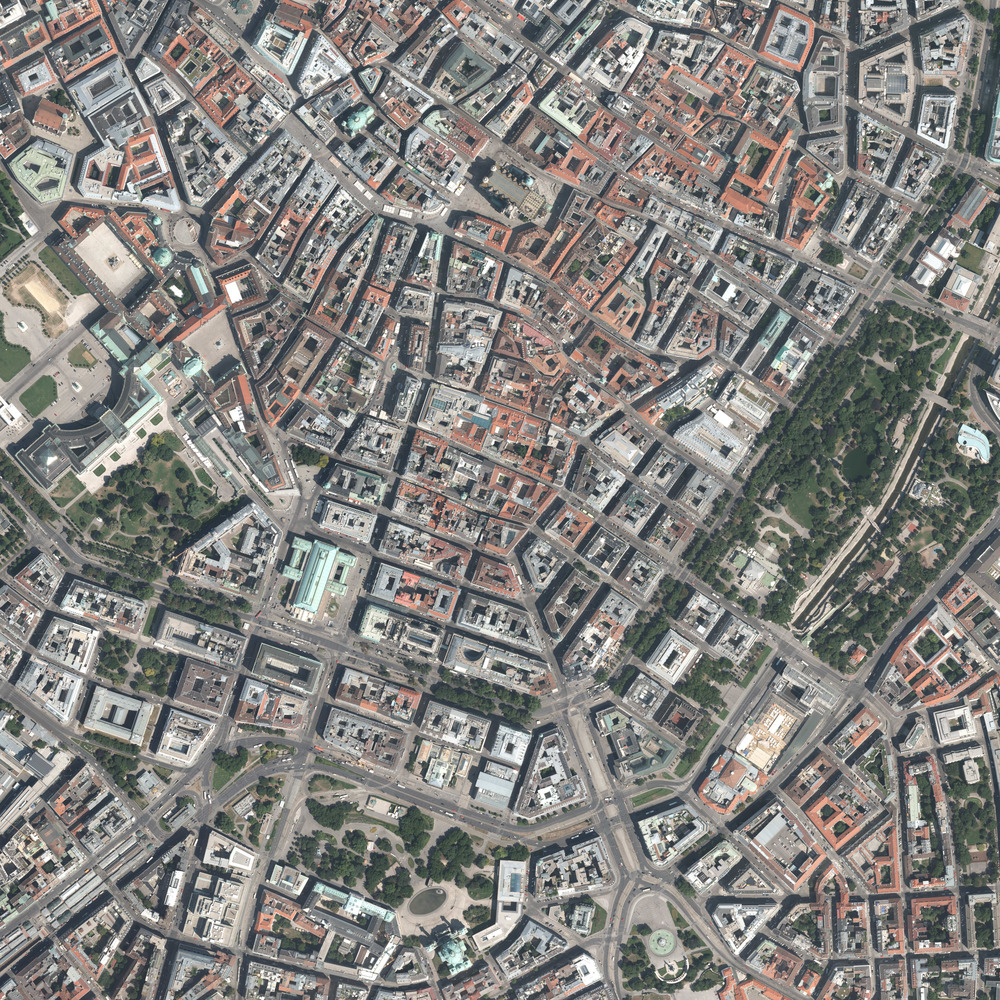
\includegraphics[width=30mm]{figs/train.jpg} &   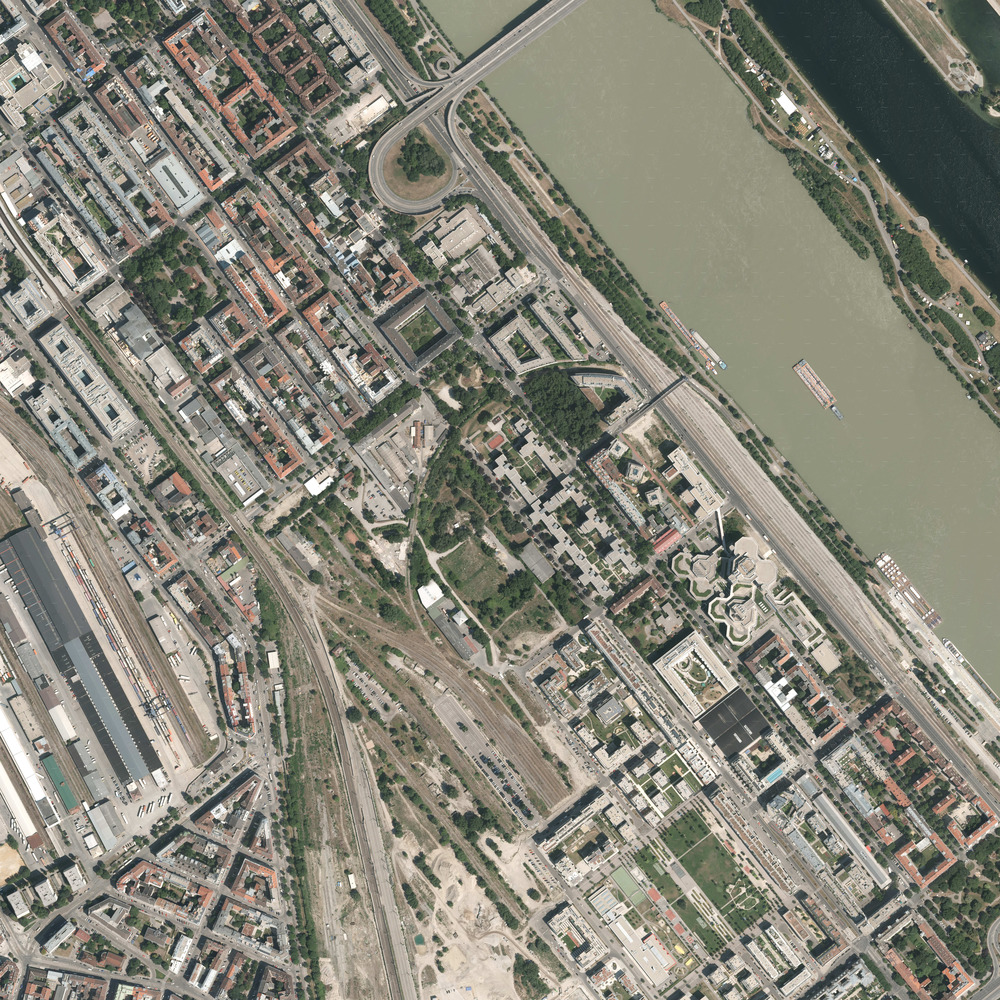
\includegraphics[width=30mm]{figs/val.jpg} &   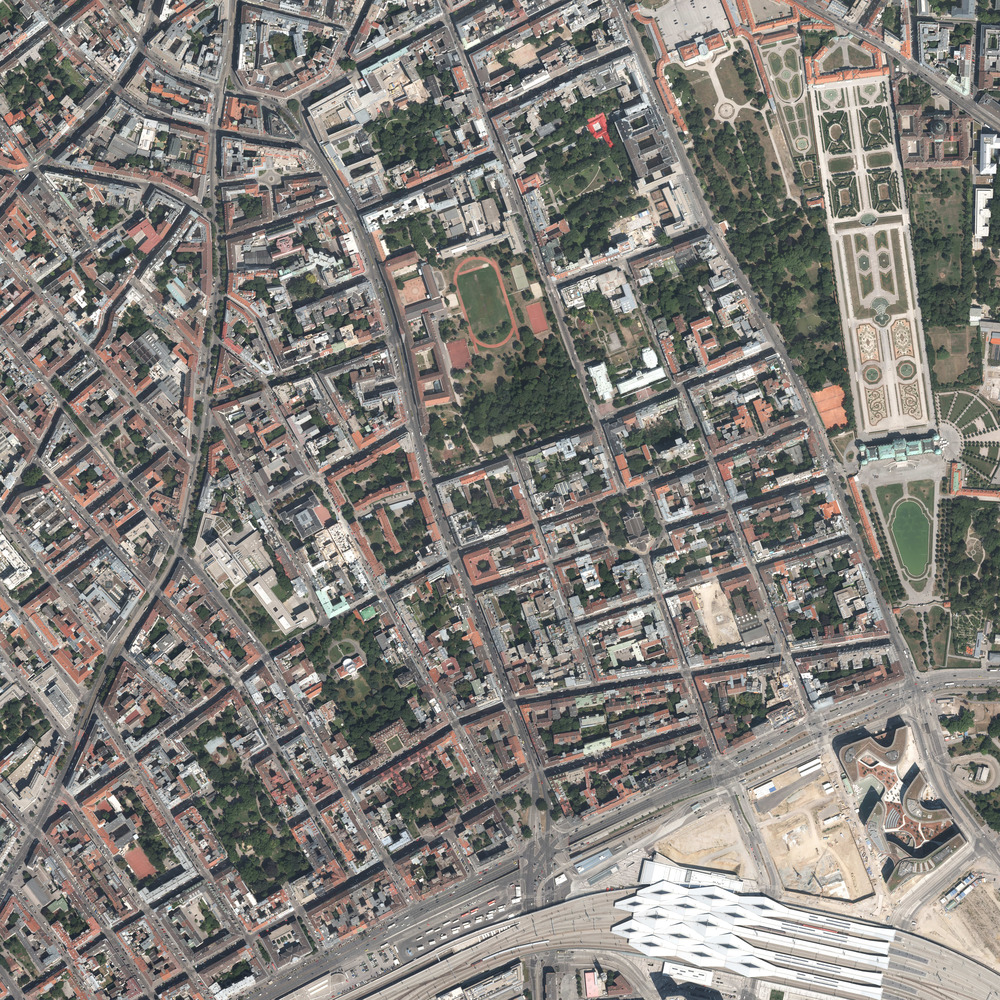
\includegraphics[width=30mm]{figs/test.jpg}\\
(a) Imagem de treinamento. & (b)Imagem de validação. & (c)Imagem de teste.  \\[6pt]
 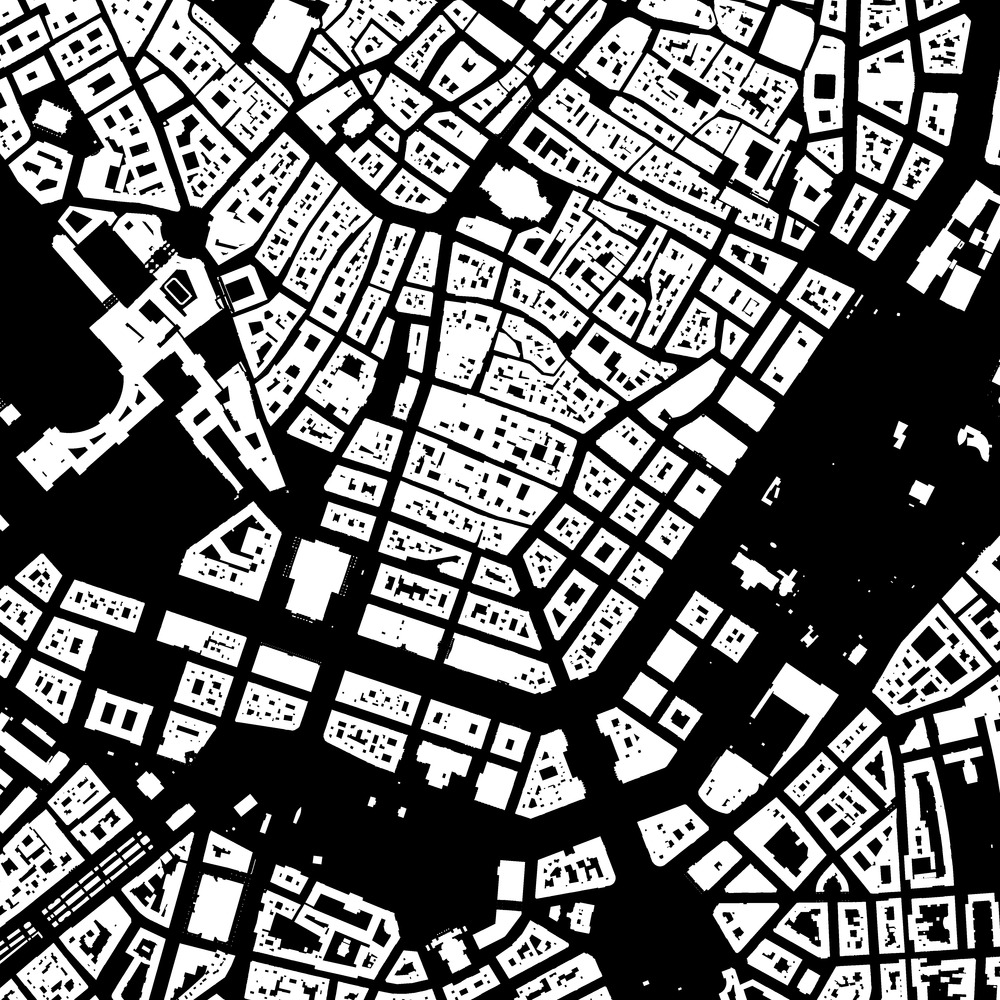
\includegraphics[width=30mm]{figs/train_label.jpg} &   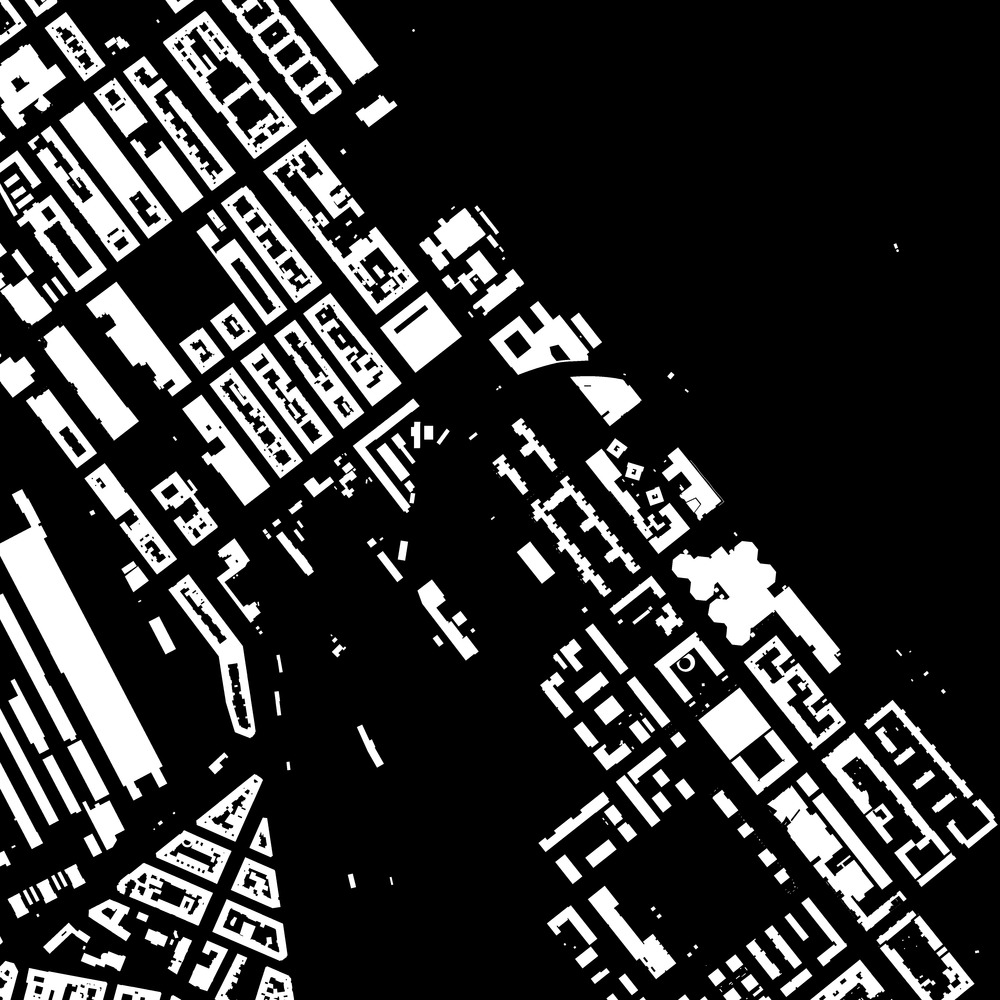
\includegraphics[width=30mm]{figs/val_label.jpg}  &   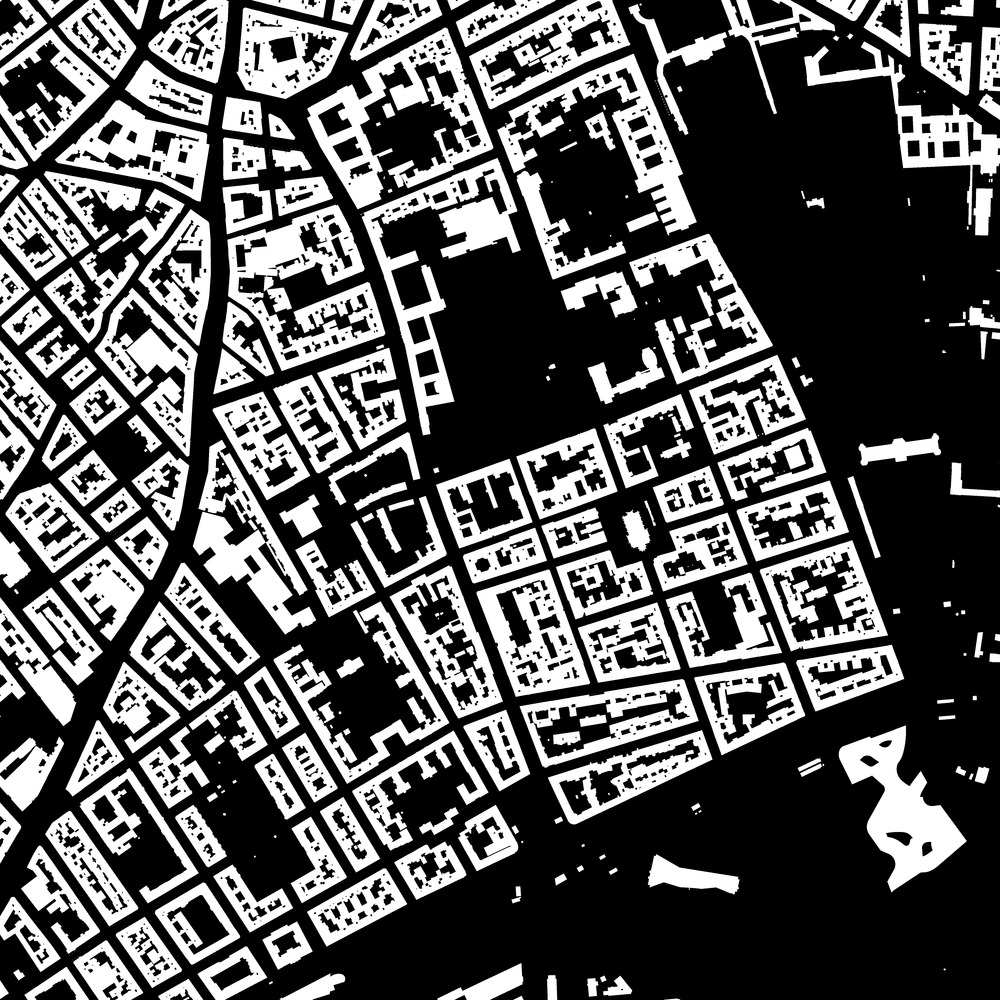
\includegraphics[width=30mm]{figs/test_label.jpg}\\
(d) Rótulo de treinamento. & (e)Rótulo de validação. & (f)Rótulo de teste.  \\[6pt]
\end{tabular}
\caption{Dataset.}
\label{fig:dataset}
\end{figure}

%-------------------------------------------------------------------------
\subsection{Requisito 1}
\subsubsection{O modelo}
Foi utilizada a técnica \textit{K-nearest Neighbors (KNN)~\cite{knn}} para a segmentação das imagens aéreas, com os descritores de textura da \textit{Grey Level Co-Ocurrence Matrix (GLCM)}~\cite{haralick} sendo ``pontos'' do conjunto de treinamento.

Essa técnica consiste em guardar todos os dados dos pontos de treinamento e rotular novos pontos baseados na proximidade com eles. Para classificar um novo ponto, o KNN busca nos $N_k$ pontos mais próximos que foram salvos e então rotula os novos pontos de acordo com a classe do conjunto de treinamento que contém a maior parte dos $N_k$ vizinhos\footnote{Alternativamente, o KNN pode ser usado para regressão. Neste caso, o resultado retornado é a média dos valores associados com os $N_k$ vizinhos mais próximos.}.

O método de classificação KNN pode ser muito efetivo, mas requer que todo o conjunto de treinamento seja salvo. Logo, ele pode usar muita memória e se tornar lento, apesar de se beneficiar do paralelismo oferecido por \textit{Field Programmable Gate Arrays (FPGAs)}.

Foram derivadas três estatísticas/\textit{features} da GLCM para serem utilizadas no KNN:
\begin{itemize}
\item Contraste: Mede as variações na GLCM e a presença de transição abrupta de níveis de cinza (bordas).
\item Energia: Fornece a soma dos quadrados dos elementos na GLCM. Também é conhecida como uniformidade ou segundo momento angular;
\item Homogeneidade: Mede a proximidade da distribuições dos elementos na GLCM com a diagonal da GLCM;
\end{itemize}
Apenas uma distância (1 pixel) e um ângulo (0 radiano) foi considerado.

Foi utilizado os 3 canais de cores da imagem com o objetivo de melhorar o resultado, visto que o pixels em nível de cinza de um prédio podem se assemelhar a pixels de um outro elemento da imagem que não corresponde a um prédio. Além disso, foi possível aumentar o número de exemplos de treinamento considerando os 3 valores de intensidade para cada pixel da imagem.

\subsubsection{Experimentos}
O KNN foi executado usando 5 e 10 vizinhos (a escolha de 5 vizinhos foi recomendada como uma boa opção por ~\cite{knn}), por motivos de comparação. Os descritores GLCM usados como \textit{features} para classificação foram obtidos dos valores dos 10734639 pixels de prédios da imagem de treino. Esses 32203917 valores de pixels foram separados em 83 matrizes para que as \textit{features} destas matrizes fossem calculadas e usadas como exemplos de treinamento para o classificador. Os pixels correspondentes a não prédios foram separados de forma similar em 87 matrizes, e alimentaram também os exemplos de treinamento do classificador. 

Para a classificação da imagem de teste foi passado uma janela de tamanho 50x50 e 100x100 na imagem. Cada uma dessas janelas foram classificadas como prédio ou não prédio, e então foi feita a contagem dos pixels que realmente são prédios. 

Assim, a acurácia foi calculada através da divisão do número de acertos pelo número total de pixels na imagem (25 milhões) e o \textit{IoU/Jaccard Index} foi calculado usando a seguinte razão: 
\begin{equation}
\centering
\text{IoU}=\frac{vp}{vp+fn+fp}\,,
\end{equation}
em que $vp$ é a quantidade de verdadeiros positivos (pixels que são prédios e foram classificados como prédios); $fn$ é a quantidade de falsos negativos (pixels que o classificador incorretamente previu como não sendo prédio); e $fp$ são os falsos positivos (pixels que o classificador incorretamente previu como sendo prédio). 
%-------------------------------------------------------------------------
\subsection{Requisito 2}
\subsubsection{O modelo}
Como segundo método de segmentação das imagens aéreas, escolhemos treinar o modelo DeepLabv3+~\cite{deeplab} com a rede MobileNetV2~\cite{mobilenet} como extrator de características de imagem.

MobileNetV2 é uma rede convolucional baseada em uma estrutura residual invertida, em que existe conexões atalho (\textit{shortcut connections}) entre camadas de gargalo (\textit{bottleneck layers}). Em vez de convoluções completas, a rede usa convoluções separáveis em profundidade (\textit{Depthwise separable convolutions}). A convolução separável em profundidade baseia-se em fatorizar a operação de convolução em duas camadas: uma convolução em profundidade que aplica um filtro para cada canal da entrada; e uma convolução por pontos (\textit{pointwise}), de tamanho 1x1, responsável por criar novas características por combinações lineares dos canais de entrada. Como resultado, são mais baratas computacionalmente sem perdas de performance significativas em relação às convoluções completas.

É aplicada a cada camada de convolução uma camada de gargalo linear, responsável por reduzir a dimensionalidade da entrada, melhorando a performance computacional da rede. Entre camadas de gargalo são usadas conexões de atalho, a fim de contribuir para a propagação do gradiente através das camadas, permitindo o treinamento de redes mais profundas. Tal estrutura, composta de convolução, gargalo e conexões residuais é o bloco de construção principal da MobileNetV2, cuja arquitetura pode ser resumida em uma camada convolucional inicial de 32 filtros, seguida por 19 blocos de gargalo e finalizada por mais duas convoluções e \textit{average pooling}.

O modelo DeepLabv3+, por sua vez, é uma rede codificadora-decodificadora (\textit{encoder-decoder}), no qual o módulo de codificação é responsável por reduzir gradualmente o mapa de características e capturar informações semânticas complexas, enquanto o módulo de decodificação tem como objetivo recuperar gradualmente as informações espaciais.

O módulo de codificação do DeepLabv3+ aplica convoluções dilatadas para extrair as características obtidas de uma rede convolucional em resolução arbitrária - no nosso caso, as características geradas pela MobileNetV2. Convoluções dilatadas permitem o controle da resolução e do campo de visão da entrada, generalizado a operação de convolução~\cite{deeplab1}. O mapa de características final do módulo de codificação possui 256 canais, permitindo a captura de informações semânticas de alto nível.

Já a parte de decodificação consiste no aumento gradual da resolução do mapa de características obtido do módulo de codificação combinado com a concatenação do mapa de características de baixo nível de resolução correspondente da MobileNetV2 e camadas de convolução. A arquitetura final do DeepLabv3+ é ilustrada pela Figura~\ref{fig:deeplab}.

\begin{figure}[htb]
\centering
\bmvaHangBox{\fbox{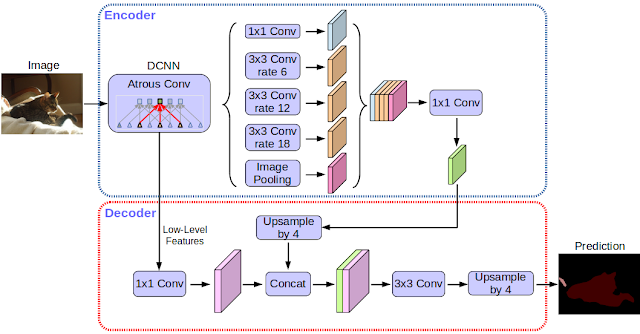
\includegraphics[width=0.5\textwidth]{figs/deeplab3+.png}}}
%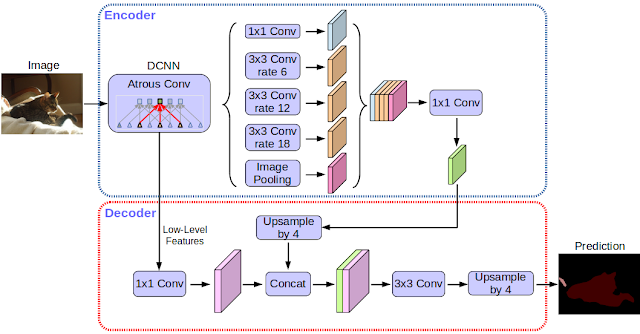
\includegraphics[width=0.8\textwidth]{figs/deeplab3+.png}
\caption{Arquitetura DeepLab3+. DCNN corresponde ao MobileNetV2. \textit{Atrous Conv} representa as convoluções dialtadas, sendo \textit{rate} o fator de dilatação. Imagem retirada de~\cite{deeplab}.}
\label{fig:deeplab}
\end{figure}

Utilizamos uma implementação em Keras do modelo descrito disponível no seguinte repositório: \url{https://github.com/bonlime/keras-deeplab-v3-plus}.

\subsubsection{Experimentos}
%FALAR DOS HIPERPARAMETROS, DOS CENARIOS E DOS CALLABLES%
Avaliamos o modelo no teste em nove cenários diferentes, envolvendo três variáveis: o tamanho da entrada, o uso de pesos pre-treinados e, neste último caso, se fixariamos os pesos do extrator de características, isto é, da MobileNetV2.

A imagem de treinamento original é de 5000x5000 pixeis, o que acarreta dois problemas. Primeiramente, não caberia na memória da GPU. Em segundo lugar, dificilmente a rede apresentaria um bom desempenho com apenas um exemplo de treinamento. Assim, resolvemos fazer experimentos dividindo as imagens de treino originais em: 2500 imagens de tamanho 100x100; 625 de tamanho 200x200; e 400 de tamanho 250x250. A intuição é que haja um trade-off entre quantidades de exemplos e tamanho da imagem, afinal, quanto maior a imagem maior a carga semântica.

Para cada um desses três tamanhos de imagem, treinamos três modelos diferentes: um com pesos inicializados aleatoriamente; um com pesos pre-treinados no dataset COCO~\cite{coco}; e outra também com pesos pre-treinados, mas com os pesos das camadas do extrator de características fixados. Espera-se que o modelo apresente melhor resultados nos dois últimos casos, uma vez que o uso de pesos pre-treinados, um caso de transferência de aprendizado, empiricamente resulta em modelos com maior capacidade de generalização.

Para cada um dos nove cenários treinamos com \text{batches} de tamanho 16, no caso de pesos do extrator fixados, e quatro nos demais casos. Como otimizador usamos \textit{Stochastic Gradient Descent} com \text{momentum} 0.9 e corte de gradientes com norma superior a um. A taxa de aprendizado tem como valor inicial 0.1, diminuindo pela metade após cinco \textit{epochs} sem diminuição da função de custo, que é a função de entropia cruzada binária. Sejam $p$ a previsão da rede e $y$ o rótulo que se deseja prever, a função de entropia cruzada binária é

\begin{equation}
    \textit{cross-entropy} = -{(y\log(p) + (1 - y)\log(1 - p))}\,.
\end{equation}


Cada modelo foi treinado em um máximo de 100 \textit{epochs}, sendo que o treinamento é interrompido após 50 \textit{epochs} sem melhoria da acurácia do conjunto de validação. Por fim, salvamos o modelo apenas quando houvesse melhora do coeficiente de Jaccard no conjunto de validação.

%-------------------------------------------------------------------------
\section{Resultados}
\label{sec:res}

%-------------------------------------------------------------------------
\subsection{Requisito 1}
\label{res:req1}
A Tabela~\ref{tab:results1} exibe os valores de acurácia e de coeficiente de Jaccard na imagem de teste para os 4 cenários.

\begin{table}[htb]
    \centering
    \begin{tabular}{c|c|c}
        Modelo & Acurácia & IoU \\
        \hline
        janelaTamanho-50-rgb-vizinhos-5 & 0.679340 & 0.370197 \\
        janelaTamanho-100-rgb-vizinhos-5 & 0.664897 & 0.352915 \\
        janelaTamanho-50-grey-vizinhos-5 & 0.679874 & 0.366998 \\ 
        janelaTamanho-50-rgb-vizinhos-10 & 0.548790 & 0.274196 \\
    \end{tabular}
    \caption{Resultados no conjunto de teste usando o método 1.}
    \label{tab:results1}
\end{table}

A Figura~\ref{fig:results1} mostra as saídas dos modelos usando janela de tamanho 50 e 100 em rgb com 5 vizinhos para o \textit{KNN}; usando janela de tamanho 50 em tons de cinza com 5 vizinhos e janela de tamanho 50 em rgb com 10 vizinhos.

\begin{figure}[htb]
\begin{tabular}{ccccc}
  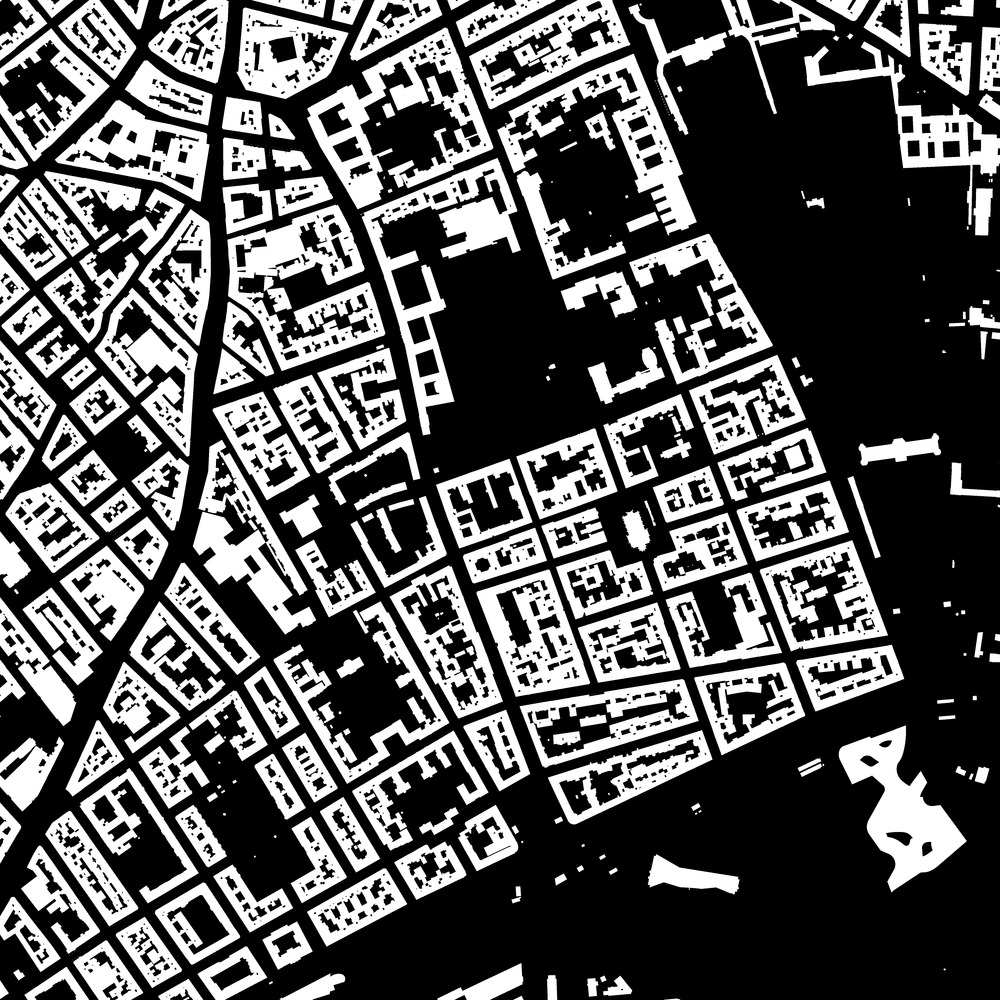
\includegraphics[width=20mm]{figs/test_label.jpg} &  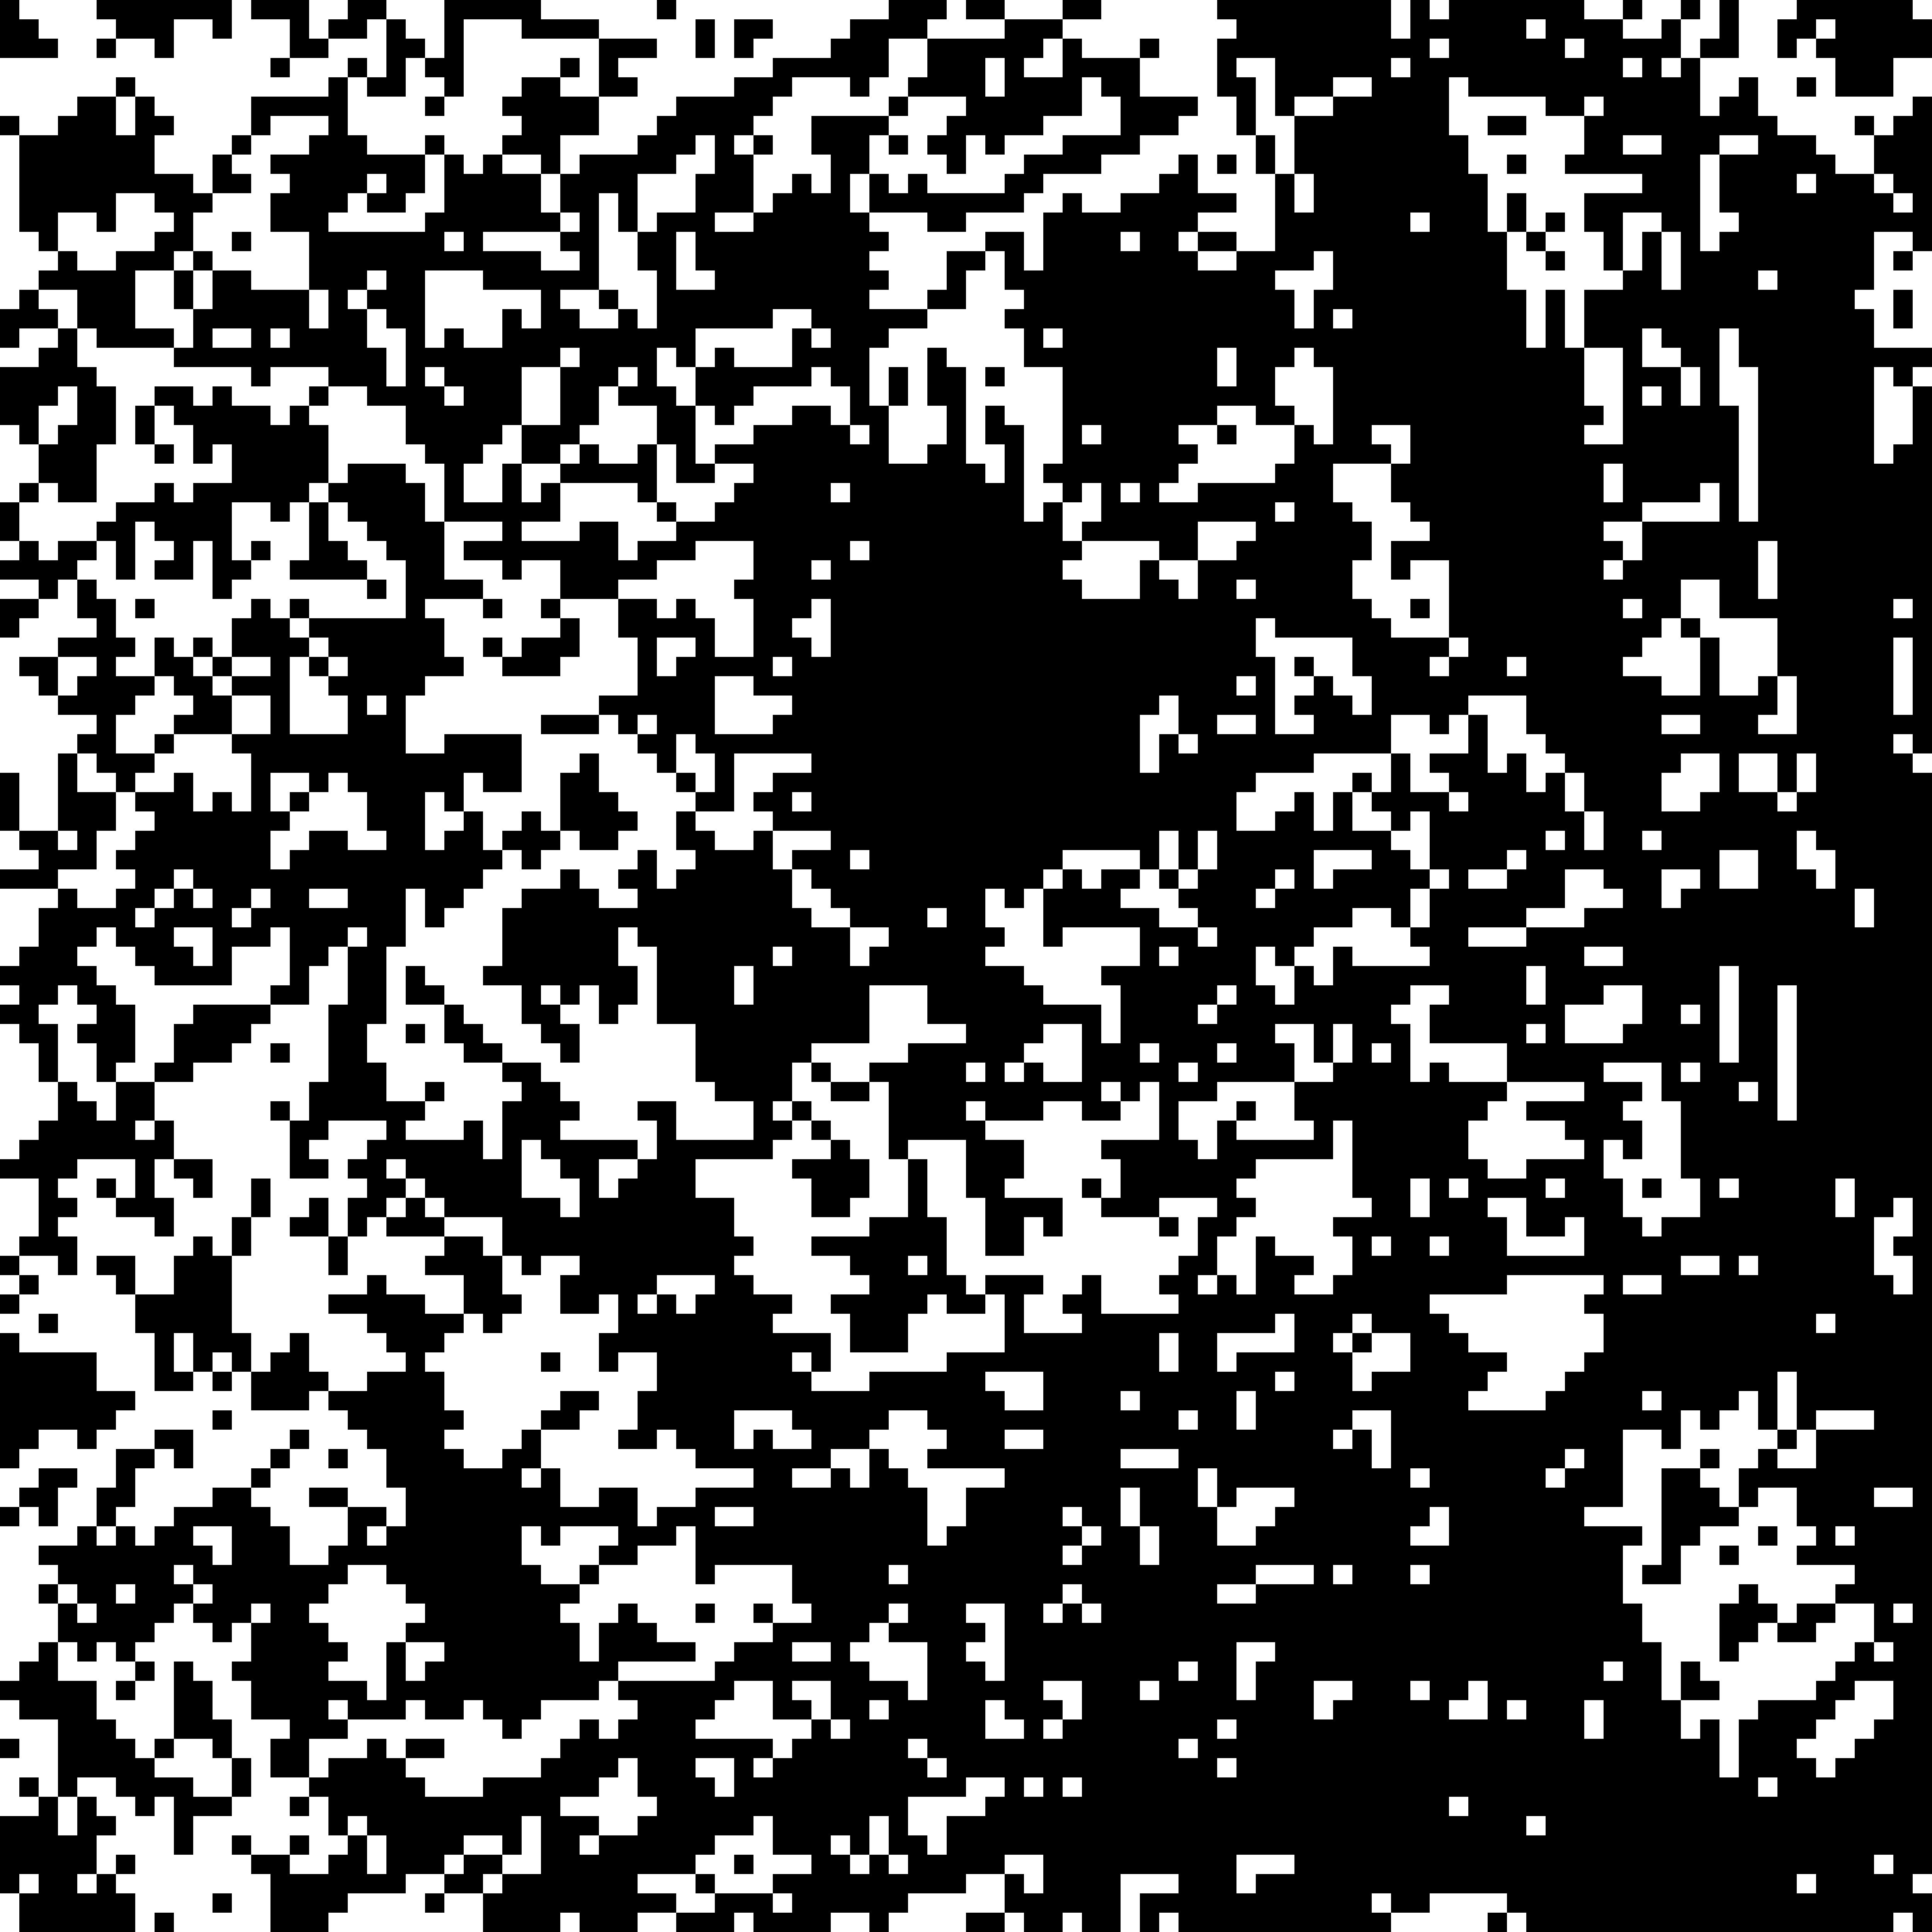
\includegraphics[width=20mm]{figs/prev_teste50.jpg} &   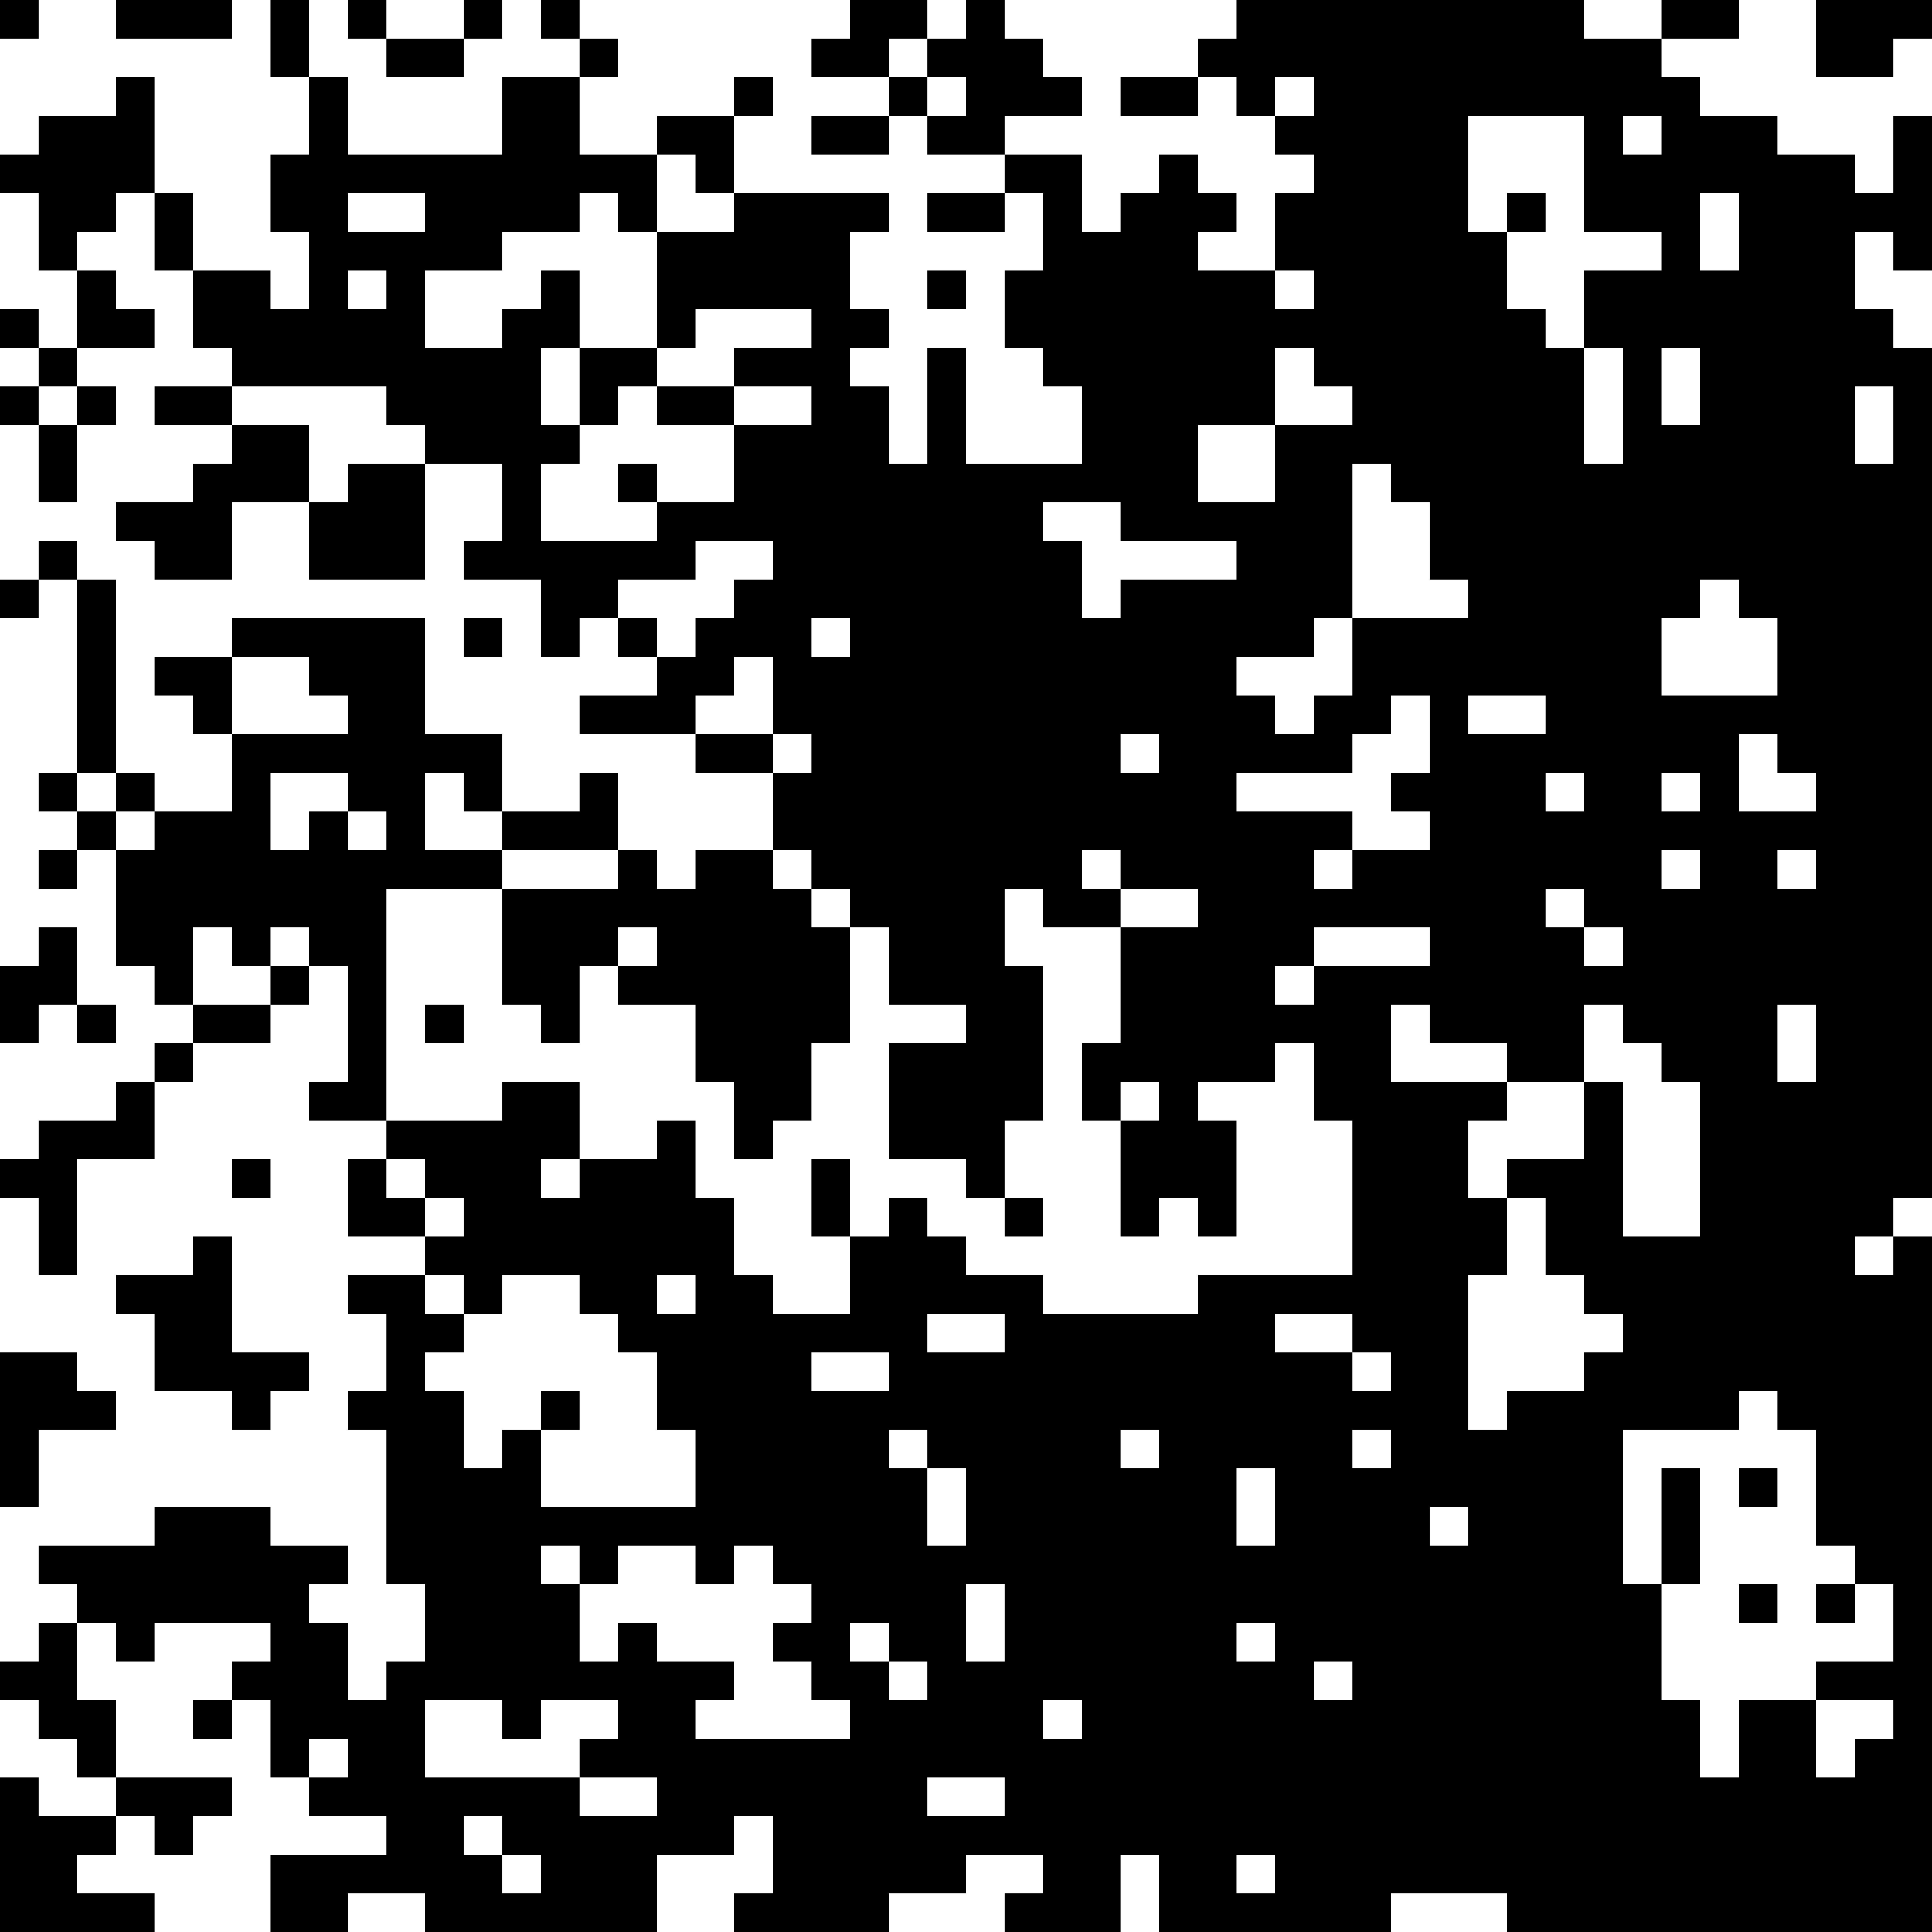
\includegraphics[width=20mm]{figs/prev_teste100.jpg} &  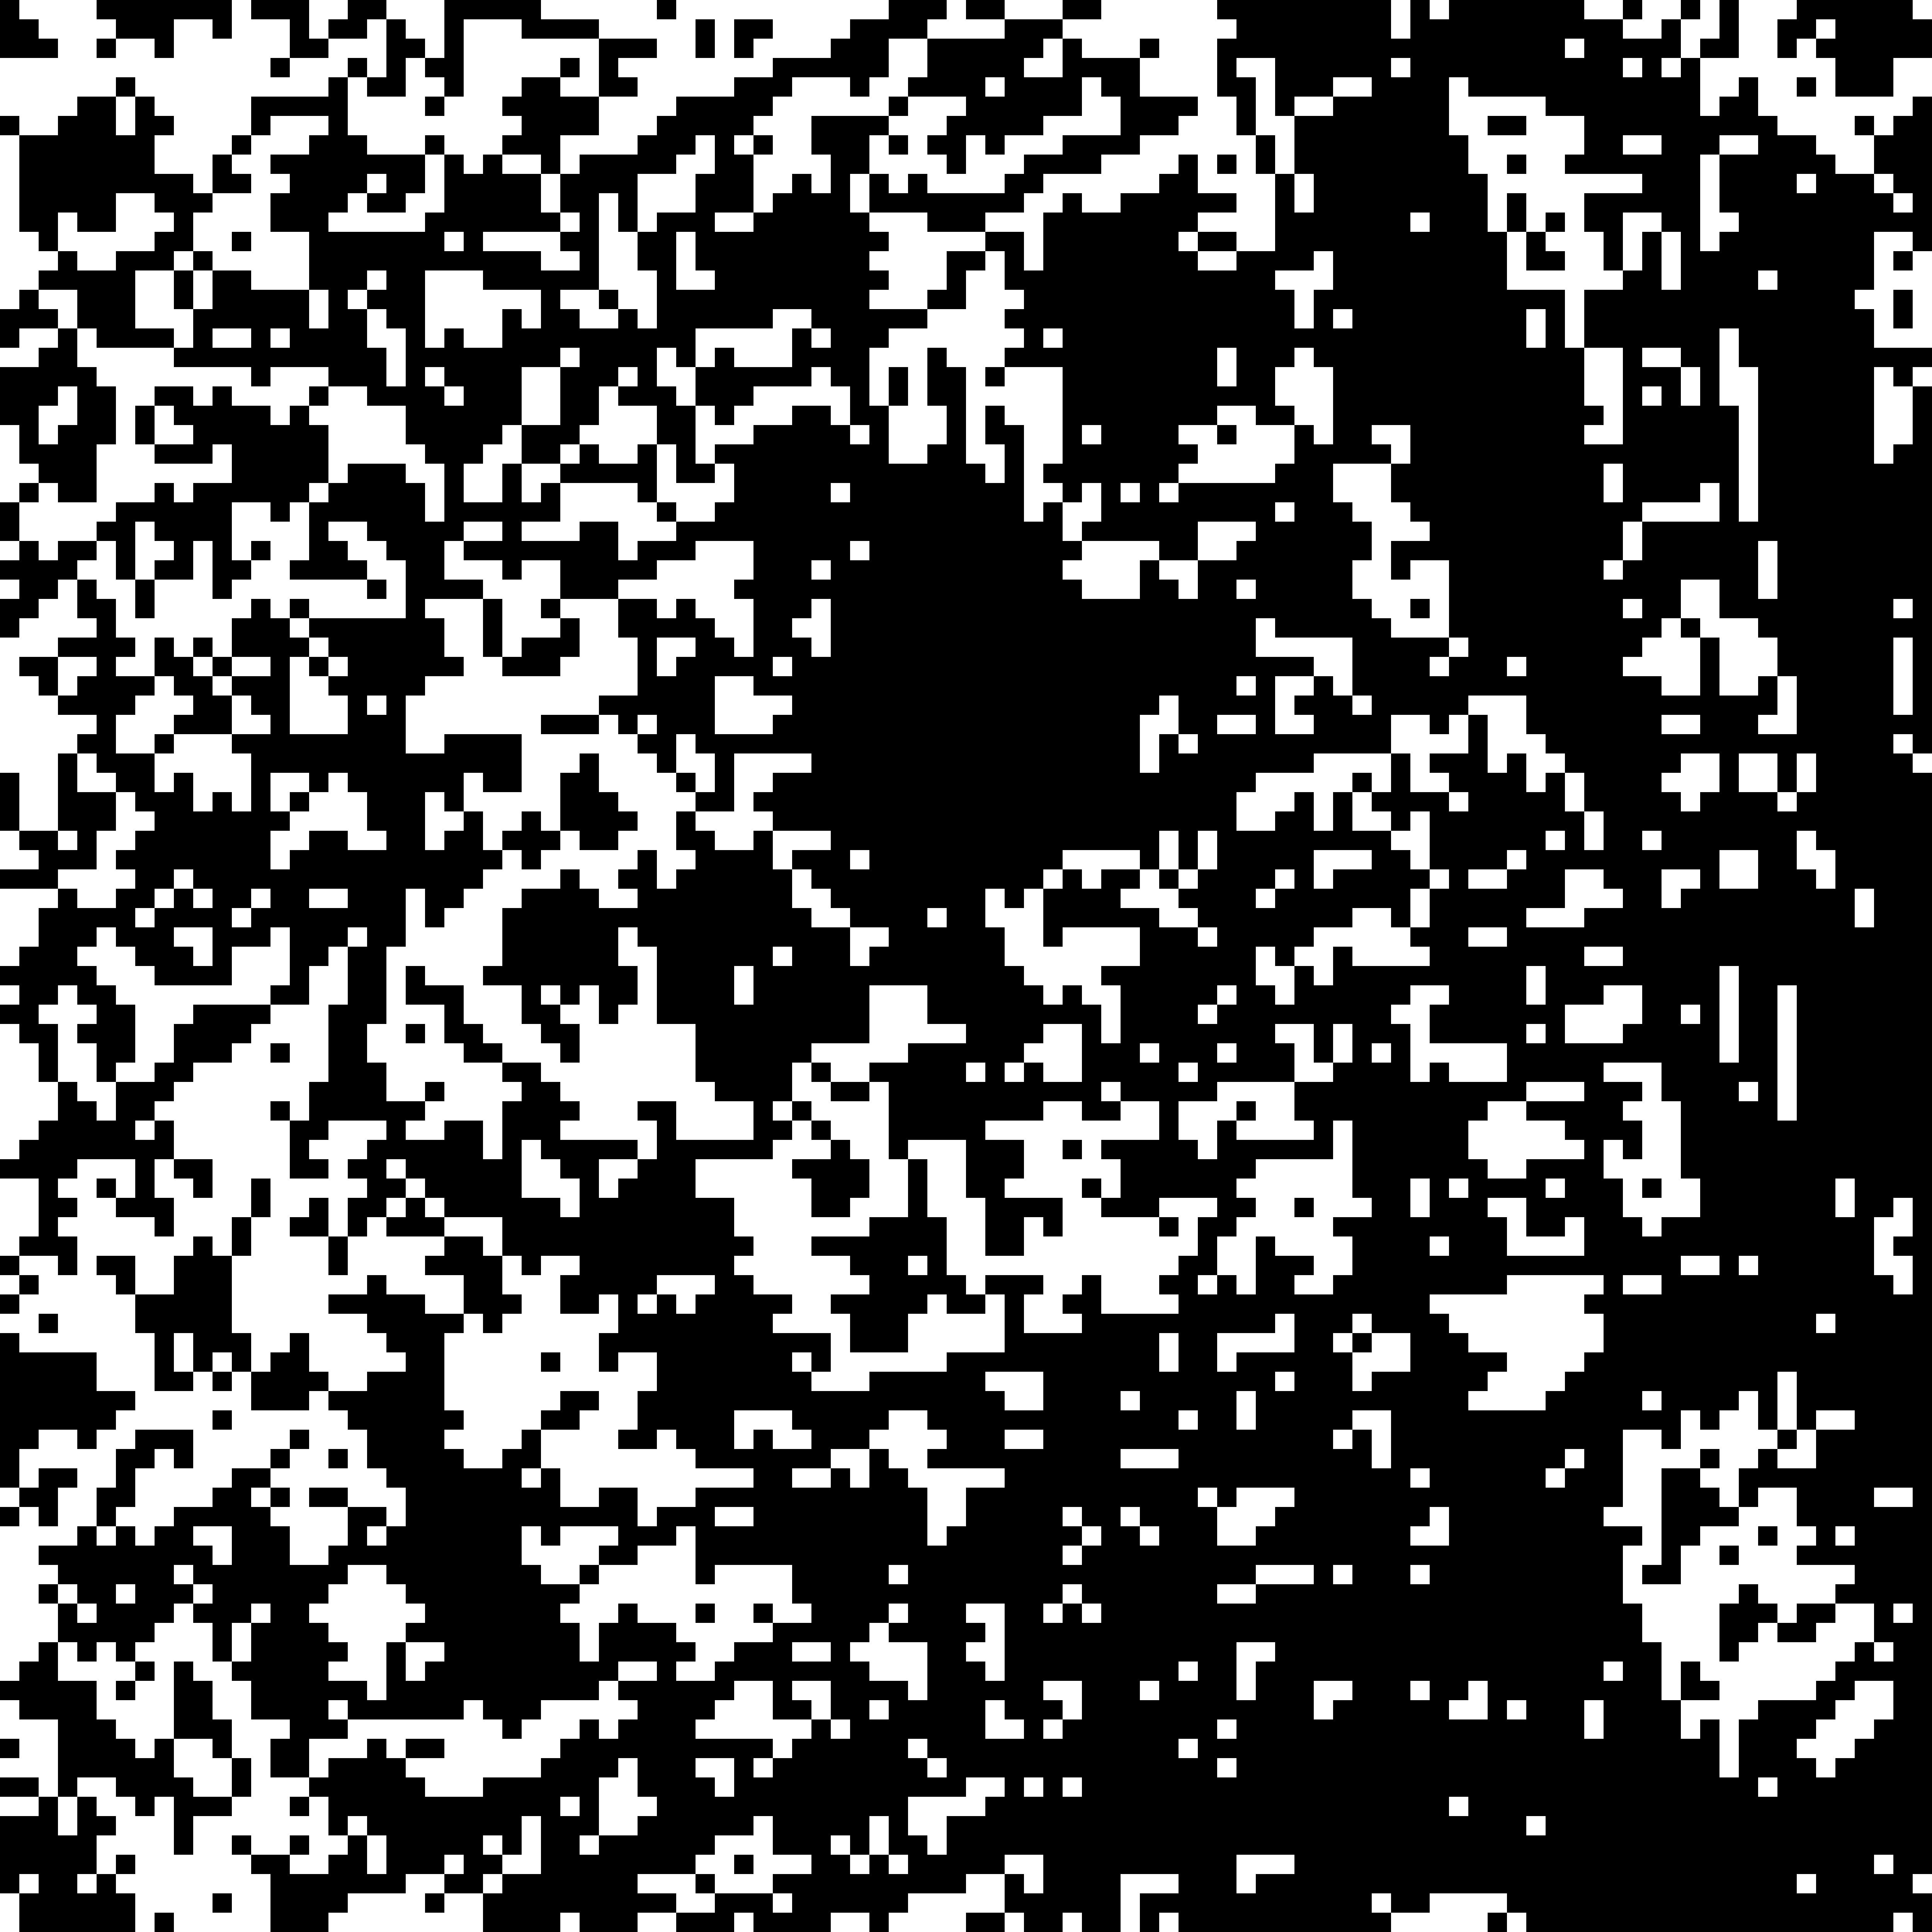
\includegraphics[width=20mm]{figs/prev_teste_gray.jpg} & 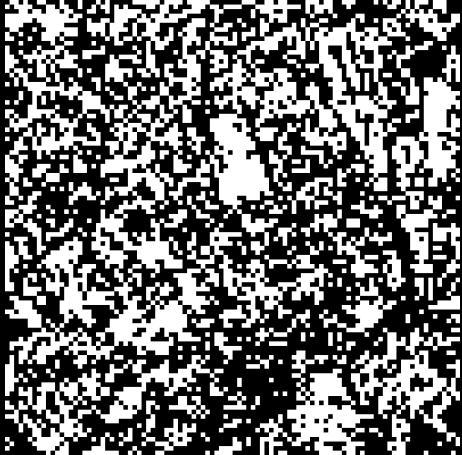
\includegraphics[width=20mm]{figs/neighbors10.jpg} \\ 
(a) Rótulo & (b) Modelo 1 & (c) Modelo 2. & (d) Modelo 3 & (e) Modelo 4. \\[6pt]
\end{tabular}
\caption{Resultados do Requisito 1.}
\label{fig:results1}
\end{figure}

O programa demorou 4 minutos para ser executado ao usar janela de tamanho 100, e 5 ao usar janela de tamanho 50.
%-------------------------------------------------------------------------
\subsection{Requisito 2}
%EXIBIR PRED E LABEL PRO MELHOR RESULTADO, ALEM JACCARD E ACCURACY PRA CADA UM DOS CENARIOS NO TESTE%

A Tabela~\ref{tab:results2} exibe os valores de acurácia e de coeficiente de Jaccard na imagem de teste para cada um dos nove cenários.

\begin{table}[htb]
    \small
    \centering
    \begin{tabular}{l|c|c}
        Modelo & Acurácia & IoU \\
        \hline
        semPretreino-naoFixo-100 & 0.86 & 0.54 \\
        preTreino-Fixo-100 & 0.65 & 0.09 \\
        preTreino-naoFixo-100 & \textbf{0.88} & 0.56 \\ 
        semPretreino-naoFixo-200 & 0.79 & 0.54 \\
        preTreino-Fixo-200 & 0.55 & 0.24 \\
        preTreino-naoFixo-200 & \textbf{0.88} & \textbf{0.64} \\
        semPretreino-naoFixo-250 & 0.84 & 0.59 \\
        preTreino-Fixo-250 &  0.35 & 0.33 \\
        preTreino-naoFixo-250 & \textbf{0.88} & \textbf{0.64} \\
    \end{tabular}
    \caption{Resultados no conjunto de teste.}
    \label{tab:results2}
\end{table}

A Figura~\ref{fig:results2} mostra a imagem de teste, sua imagem de rótulo, e as saídas dos modelos com pre-treino, sem pesos fixos, e treinados com imagens de tamanho 200 (modelo 1) e 250 (modelo 2), por terem obtidos os melhores resultados de acurácia e de coeficiente de Jaccard. 

\begin{figure}[htb]
\centering
\begin{tabular}{cccc}
  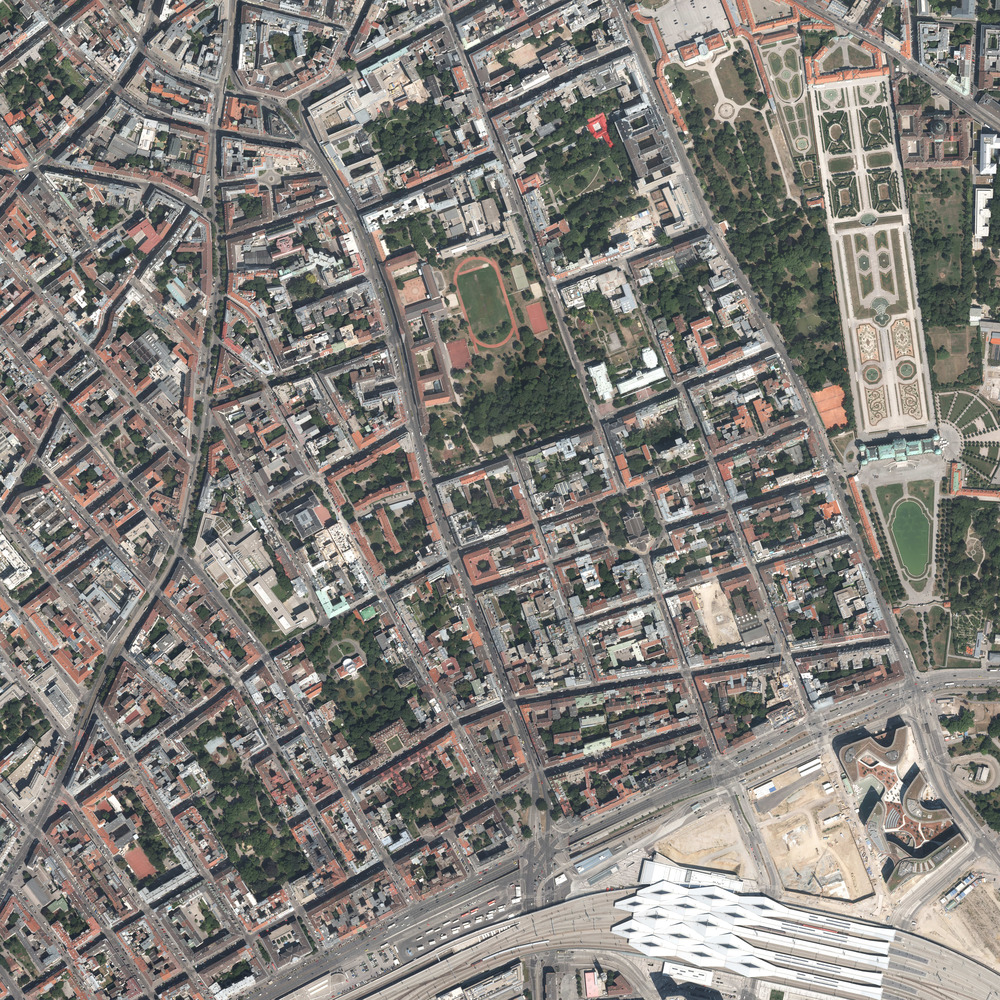
\includegraphics[width=20mm]{figs/test.jpg} &   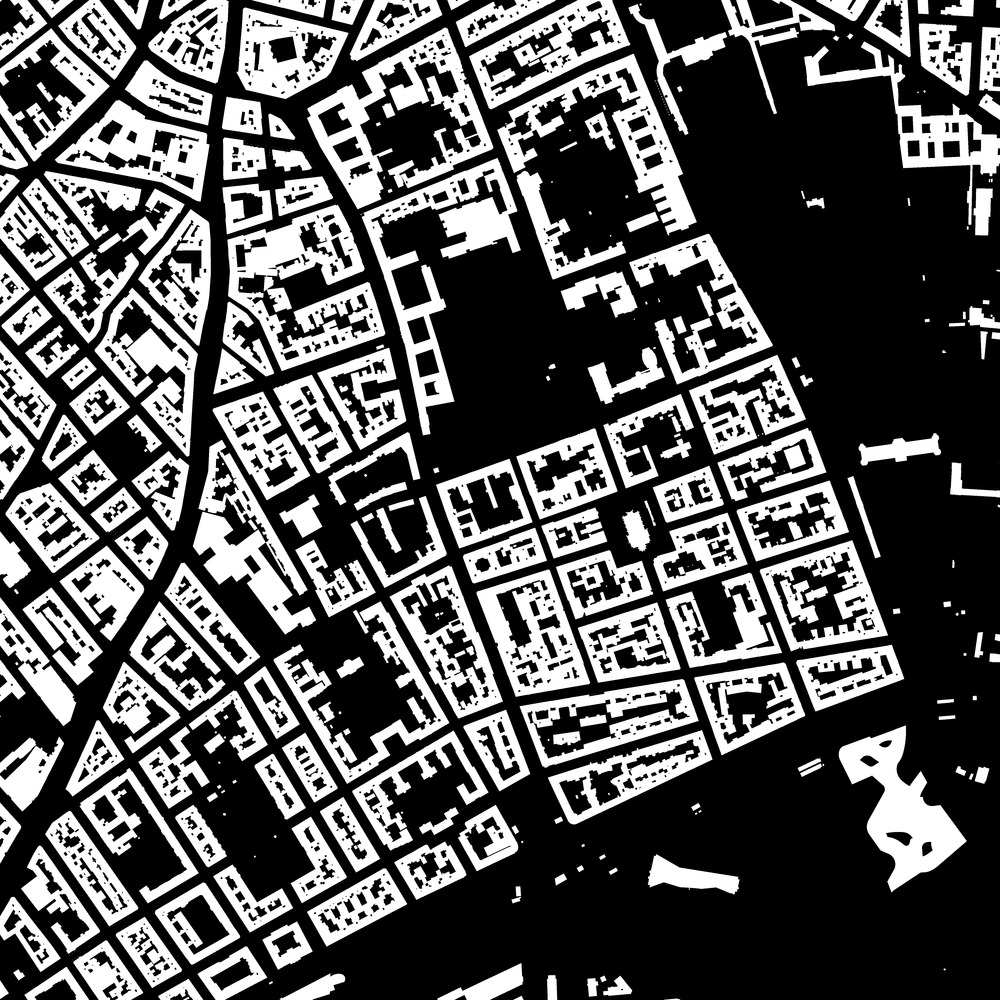
\includegraphics[width=20mm]{figs/test_label.jpg} &   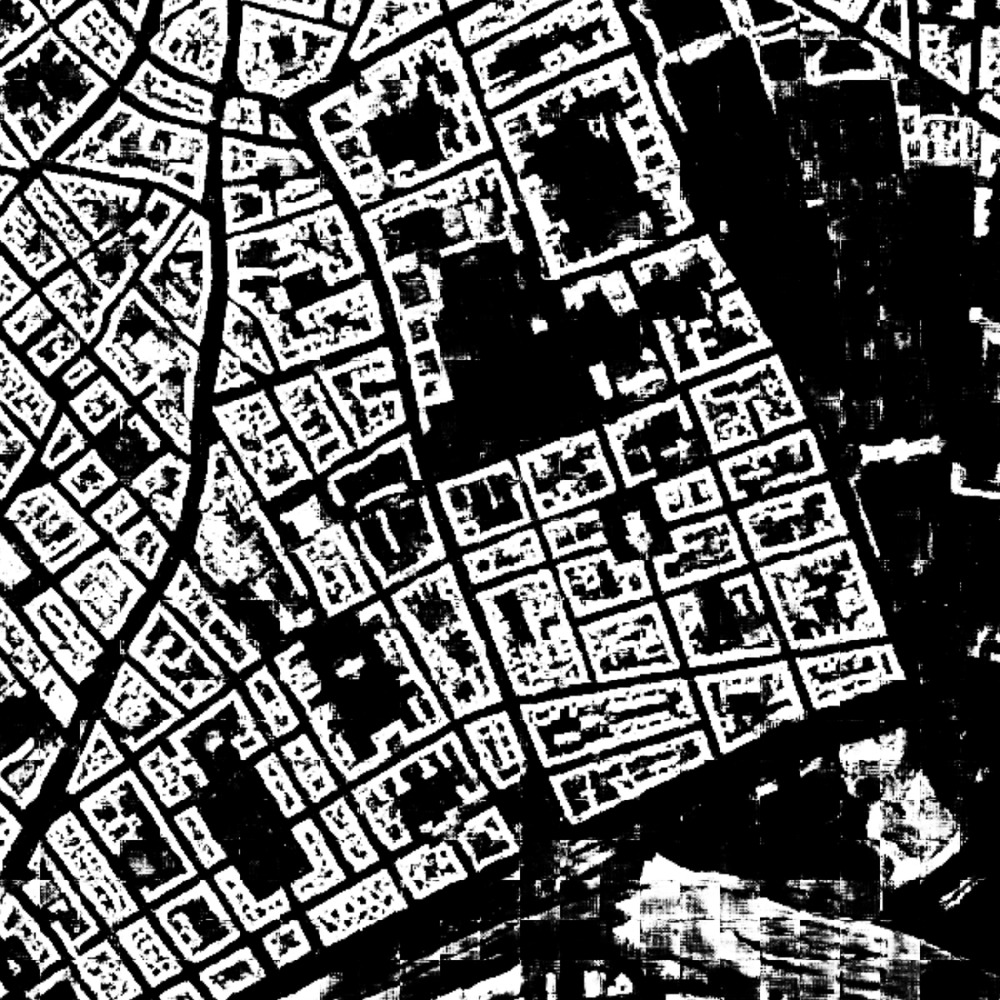
\includegraphics[width=20mm]{figs/pred200.jpg} & 
  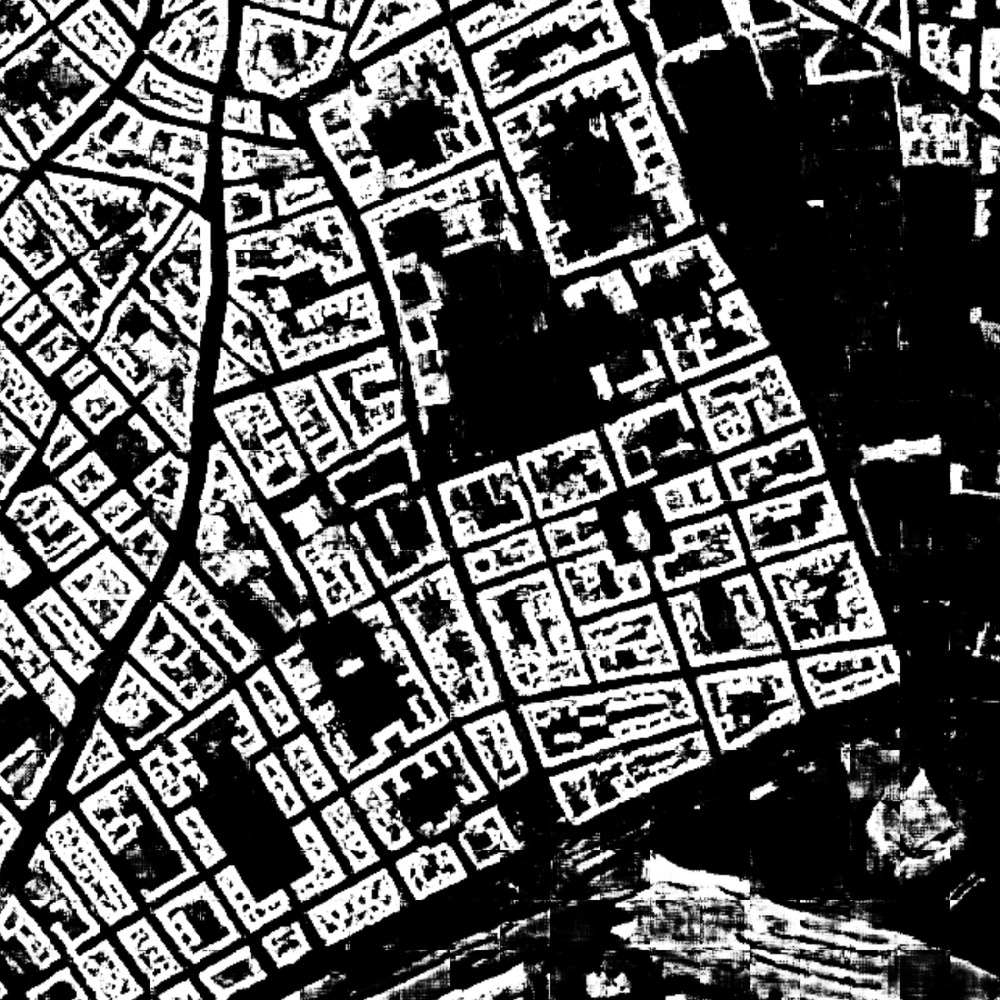
\includegraphics[width=20mm]{figs/pred250.jpg} \\ 
(a) Imagem. & (b) Verdade. & (c) Previsão 1. & (d) Previsão 2. \\[6pt]
\end{tabular}
\caption{Resultados do Requisito 2.}
\label{fig:results2}
\end{figure}

%-------------------------------------------------------------------------
\section{Discussão e Conclusões}
\label{sec:conc}
%BONS RESULTADOS, CUSTO COMPUTACIONAL, DESNECESSIDADE DE FEATURE ENGINEERING, TRANSFER LEARNING APRENDE COM POUCOS EXEMPLOS, TRADE OFF TAMANHO DA IMAGEM x NUMERO DE EXEMPLOS, MELHORIAS: DATA AUGMENTATION, TREINO NO CONJUNTO INTEIRO% 
\subsection{Requisito 1}
Nota-se pela Tabela ~\ref{tab:results1} que o uso de 10 vizinhos para o algoritmo \textit{KNN} prejudicou bastante a classificação. O que faz sentido, visto que aumentar o número de vizinhos diminui a capacidade do modelo. A grosso modo, a capacidade do modelo descreve o quão complexa é a relação que o modelo pode modelar. Um modelo com maior capacidade tem capacidade de modelar mais relacionamentos entre mais variáveis do que um modelo com menor complexidade.

Além disso, o uso da janela de tamanho 100 afetou de forma significativa o resultado visual na imagem de teste. Apesar da acurácia ter diminuído em apenas 1\% e o IoU em 2. Este resultado negativo já era esperado, visto que estamos classificando janelas inteiras como pertencentes a prédios ou não. Entretanto, o uso de janelas muito pequenas também não ajudou, visto que precisamos de mais pixels para obter descritores mais precisos e que caracterizam melhor o conjunto em questão.

O uso da imagem de teste em nível de cinza em vez das cores rgb pouco alterou o resultado visual e estatísticos. O que indica que os pixels referentes aos prédios mantém boa distinção com os pixels referentes a não prédios, mesmo em nível de cinza.

Para melhora do algoritmo de Machine Learning utilizado poderia ter sido utilizado \textit{cross-validation} para melhor ajuste dos parâmetros. Entretanto, os resultados provavelmente não seriam muito diferentes dos obtidos.

\subsection{Requisito 2}
O método elaborado no Requisito 2 apresentou bons resultados. A Figura~\ref{fig:results2} demonstrou que as previsões dos melhores modelos são extremamente semelhantes ao rótulo da imagem teste. A maior fonte de erro se deu no canto inferior direito da imagem. Nota-se da imagem  original que nessa região há uma espécie de construção sobre trilhos de trem, os quais não são considerados como edifícios pelo \textit{ground truth}, embora sejam muito semelhantes a prédios quando vistos de cima.

Temos como vantagem do uso de aprendizado profundo a desnecessidade de engenharia de características - a própria rede o faz, podendo atingir resultados superiores a características criadas por humanos. Como contrapartida, necessita-se de uma grande quantidade de exemplos de treinamento. Entretanto, isso pode ser mitigado pelo uso de transferência de aprendizado, como o fizemos ao usar pesos pre-treinados.

Percebe-se que os modelos com pesos do extrator de características fixos apresentaram baixa performance. Isso pode ser explicado, talvez, em razão da diferença do domínio de imagens aéreas do domínio onde foram treinados os pesos, que são imagens de objetos em contextos ordinários. Não obstante, ficou claro que o uso de pesos pre-treinados melhorou os resultados quando permitiu-se o \textit{fine-tuning} em todas as camadas da rede. Quanto ao \textit{trade-off} número de exemplos x tamanho das imagens, nota-se que modelos treinados com imagens de diferentes tamanhos apresentaram aproximadamente a mesma performance, com uma ligeira vantagem de imagens maiores quanto ao índice Jaccard.

Um problema do Requisito 2 é o alto custo computacional: foi necessária um pouco mais de uma hora para treinar cada um dos modelos. Caso não fosse usada uma GPU tal tempo seria muito superior. Por outro lado, uma vez treinada a rede a inferência é rápida, sendo necessário menos de um minuto para classificar os 25 milhões de pixeis da imagem de teste sem o uso de GPU e contando o tempo do carregamento inicial da rede.

Como melhoria, há a possibilidade do uso de técnicas de aumento de dados (\textit{data augmentation}) para aumentar o número de exemplos. Isso inclui transformações aleatórias nas imagens, como rotação, inversões horizontais e verticais, e zooms. Como trabalho futuro mostra-se interessante o treinamento da rede no conjunto inteiro de imagens aéreas com o uso de \textit{data augmentation}.

\clearpage
\bibliography{refs}
\end{document}
